% ============================================================================
%  TECS submission draft
%  Transformations and Trajectories of a Content-Addressed State Machine
% ----------------------------------------------------------------------------
%  Build:  pdflatex tecs_state_machine_trajectory.tex   (run twice)
%  Compiles against companion.tex's conventions/notation.
%  NOTE: author list and affiliations mirror the companion note; confirm before
%        submission.
% ============================================================================
\documentclass[11pt,a4paper]{article}

\usepackage[utf8]{inputenc}
\usepackage[T1]{fontenc}
\usepackage{amsmath,amssymb,amsthm}
\usepackage{booktabs}
\usepackage{graphicx}
\usepackage{array}
\usepackage{tikz}
\usetikzlibrary{arrows.meta,positioning,fit,backgrounds}
\usepackage{hyperref}
\usepackage[margin=1in]{geometry}
\usepackage{enumitem}
\usepackage{xcolor}
\definecolor{hlblue}{RGB}{0,80,160}
\hypersetup{colorlinks=true,linkcolor=hlblue,urlcolor=hlblue,citecolor=hlblue}

\newtheorem{principle}{Principle}[section]
\newtheorem{definition}[principle]{Definition}
\newtheorem{proposition}[principle]{Proposition}
\newtheorem{corollary}[principle]{Corollary}
\theoremstyle{remark}
\newtheorem{remark}[principle]{Remark}

% ---- shorthands (aligned with the companion note) --------------------------
\newcommand{\Plane}{\ensuremath{\mathbb{B}}}          % bit plane
\newcommand{\Lat}{\ensuremath{\mathcal{B}}}           % HLLSet (Boolean) lattice
\newcommand{\Tok}{\ensuremath{\mathcal{T}}}           % token space
\newcommand{\HLL}{\ensuremath{H}}                     % an HLLSet
\newcommand{\xor}{\ensuremath{\Delta}}                % ring addition
\newcommand{\Reg}{\ensuremath{\mathsf{M}}}            % register count
\newcommand{\Prec}{\ensuremath{P}}                    % precision
\newcommand{\Bits}{\ensuremath{b}}                    % bits per register
\newcommand{\BSS}{\ensuremath{\mathsf{BSS}}}          % BSS measure
\newcommand{\res}{\ensuremath{\mathrm{res}}}          % residual
\newcommand{\spanof}[1]{\ensuremath{\langle #1\rangle}} % GF(2) span
\newcommand{\Tab}{\ensuremath{\mathsf{T}}}            % a turn

\title{\textbf{Transformations and Trajectories of a Content-Addressed
State Machine}\\[4pt]
\large The Emerging World Model HLLSet Architecture\\[6pt]
\normalsize (TECS submission draft)}

\author{Alex Mylnikov \and Alexandr Mylnikov Jr. \and Deependra Kumar}
\date{\today}

\begin{document}
\maketitle

\begin{abstract}
Contemporary AI systems are stateless at inference time: each request is
answered from a context window that is rebuilt from scratch, and ``memory'' is a
buffer rather than a state. We describe \texttt{ewm-state-machine}, an
engineering realization of \emph{Emerging World Models} (EWM) in which the state
itself is a content-addressed set. The state is an \textbf{HLLSet}---a compact
bit-vector sketch of a token collection over a fixed $32$K-bit plane---and every
transformation of the machine is an operation on a Boolean lattice: union joins,
intersection meets, symmetric difference is ring addition. The paper's center of
gravity is the \textbf{transformation} and the \textbf{trajectory}: a single
turn ingests a token stream, updates the working state $S(t)$ by a join, pushes
the incoming original into a GF(2) ring whose basis is \emph{monotone}
(every commit HLLSet stays in the base's span), commits the result to a
content-addressed store, and materializes tokens back for the host. We separate
the temporal roles cleanly---$S(t)$ is the emerging state, $H(t{-}1)$ the
committed base, and $D/R/N$ the departed/retained/new decomposition---and we
organize the running record as a set of \emph{frames} whose coordinates form the
state trajectory. We present the architecture (foundation crates for HLLSets and
morphisms; state crates for the store, cache, processing unit, explorer, and
side-car hosts), the transformation algebra (extension and rotation over a
moving basis, exact change of basis between commits), and a trajectory toolkit
with labeled exactness: canonical coordinates, novelty, covers, and minimal
covers. We then give the view that makes the trajectory readable: the ring basis
is a \emph{rotating coordinate system}, and each commit's top state is
decomposed in the coordinates current when it arrives---a soft key (the
projection onto each base coordinate), a hard key where the state lies in the
span, and a residual for the off-span part. The same property dictates what the
store keeps: only \emph{originals} and \emph{base HLLSets} are materialized,
while every compound---union, $D/R/N$, residual, or projection---is recorded as
a provenance-stamped \emph{view} (an expression plus the SHA-1 identifiers of
its sources) and recreated against the base current at read time. On a
$10\times10$ synthetic
clip the linear residual flags all nine scene cuts, the bit-novelty signal
separates cuts from in-scene drift by $3.75\times$, symmetric differences are
always representable in the ring, and intersections/unions/differences are the
measurable obstruction. The rotating-coordinate trajectory reads out the
transition structure directly: the basis frontier grows monotonically, $534$
coordinates re-pivot over $100$ commits, and the pre-commit residual spikes at
every scene cut. The result is a reproducible, vocabulary-agnostic
state layer that any model can use as a side-car.
\end{abstract}

\noindent\textbf{Keywords:} content-addressed state; HLLSet; Boolean lattice;
GF(2) linear algebra; state machine; trajectory; side-car memory; HyperLogLog.

% ============================================================================
\section{Introduction}
\label{sec:intro}
% ============================================================================

A language model, a vision model, or a planner is a function: it maps an input
to an output and keeps nothing. What we call its ``memory'' is a text buffer or
a key--value cache that is re-derived for every request. This is convenient, but
it means the system has no \emph{state} in the control-theoretic sense: there is
no value that is advanced, committed, and recovered; no notion of what was
retained, what departed, and what is new. Rebuilding context from scratch is
also where much of the cost and most of the failure modes of long-horizon
systems live.

This paper describes \texttt{ewm-state-machine}, a state layer built on one
unusual choice: \textbf{the state is a content-addressed set}, not a tensor. A
token stream is measured into an \textbf{HLLSet}~\cite{astesj2026,companion2026}:
a fixed-length bit vector whose set bits are the sites the tokens hashed into
($32{,}768$ bits $= 4$\,KB at the default geometry). Because subsets of a common
plane form a Boolean lattice~\cite{birkhoff1940}, every state and every
derived quantity---unions, intersections, differences, novelty, residuals---is
a node of one lattice, addressed by content (IICA: idempotent, immutable,
content-addressed). Nothing is created that was not already a node; a
computation \emph{discovers} a node by naming a lattice expression
\cite{companion2026}.

The consequence is a state machine whose transformations are cheap and exact set
operations, and whose trajectory is a sequence of nodes that can be replayed,
compared, and audited. The processing unit is stateless and disposable: it reads
a tip, ingests a turn, proposes the next state, and forgets. The state lives
\emph{outside} it, in a shareable cache and a persistent store. Recovery is a
``pop, not a rebuild'': discard the unit and its cache, restore from the tip, and
continue; uncommitted work is reprocessed, and idempotence makes that safe.

\paragraph{Contributions.}
\begin{enumerate}[leftmargin=*,nosep]
  \item \textbf{A state-machine formulation.} We give the fundamental equation
    $H(t) = (S(t), H(t{-}1), D, R, N)$ and the four ideas that make it safe
    (one universe; the morphism is the contract; the fiber is global;
    decompositions are frames)---\S\ref{sec:ewm}.
  \item \textbf{An architecture.} We describe the layered realization:
    foundation crates for HLLSets, contracts, LUTs, and morphisms; state crates
    for the content-addressed stack, the cache, the processing unit, the
    explorer, the operational graph, and the side-car hosts---\S\ref{sec:arch}.
  \item \textbf{Transformations.} We specify one turn exactly: encode, ingest,
    join, ring-push, commit, materialize. The ring basis is \emph{monotone}
    (every commit HLLSet stays in the base's span), so the span only grows
    and representability is non-decreasing; a change of basis transports
    coordinates exactly across commits---\S\ref{sec:transforms}.
  \item \textbf{Views, not stored compounds.} The same transport property fixes
    the storage discipline: only originals and base HLLSets are materialized,
    while every compound is a provenance-stamped view recreated against the base
    current at read time---\S\ref{sec:views}.
  \item \textbf{Trajectories and tools.} We formalize readings (frames) and
    their coordinates as the state trajectory, and we present a toolkit with
    explicit exactness: canonical coordinates, novelty, bit-novelty via covers,
    and minimal covers for context compression---\S\ref{sec:trajectory}.
  \item \textbf{Rotating coordinates and the top-state decomposition.} We show
    that the ring basis is a rotating coordinate system and decompose each
    commit's top state in the coordinates current when it arrives---soft key,
    hard key, and residual---which makes the transition structure readable as a
    coordinate--time matrix (base coordinates on $Y$, commits on $X$)---%
    \S\ref{sec:rotating}.
  \item \textbf{Reproducible evidence.} On a $10\times10$ scene clip the
    residual detects all nine cuts, the bit-novelty signal separates cuts from
    in-scene drift by $3.75\times$, and the representability laws are measured
    (symmetric difference $394/394$ in span; intersection/union/difference
    $0/394$)---\S\ref{sec:experiments}.
\end{enumerate}

The paper is deliberately engineering-first. The mathematics is kept to the
minimum needed to say what the machine does and why it is safe; the full
lattice/world theory is in the companion note~\cite{companion2026} and the main
EWM paper~\cite{ewm2026}.

% ============================================================================
\section{HLLSets and the Boolean lattice}
\label{sec:roots}
% ============================================================================

\subsection{What an HLLSet is}

An \textbf{HLLSet} is a compact sketch of a token collection. Instead of storing
tokens, it stores a fixed-length bit vector whose set bits are the
\emph{measurement sites} the tokens hashed into. The geometry is
\emph{soldered}~\cite{astesj2026,companion2026}: precision $\Prec$ fixes the
register count $\Reg = 2^{\Prec}$; each register occupies $\Bits$ bits; a token
$t$ is hashed once and decomposed into a register index and a trailing-zero
state,
\begin{equation}
\label{eq:position}
\mathrm{reg}(t) = h(t) \bmod \Reg,
\qquad
\mathrm{tz}(t) = \mathrm{clamp}\!\left(\mathrm{trailing\_zeros}(h(t)\gg\Prec),\,0,\,\Bits-1\right),
\end{equation}
naming a single \textbf{bit address}
\begin{equation}
\label{eq:bit}
\mathrm{bit}(t) = \mathrm{reg}(t)\cdot\Bits + \mathrm{tz}(t)
\;\in\;\{0,\dots,\Reg\cdot\Bits-1\}.
\end{equation}
With the defaults $\Prec=10$, $\Bits=32$, the plane has
$\Reg\cdot\Bits = 32{,}768$ bits (4\,KB packed). The sketch of a token collection
$A\subseteq\Tok$ is
\begin{equation}
\label{eq:sketch}
\HLL(A) = \bigcup_{t\in A}\{\mathrm{bit}(t)\},
\end{equation}
so a collection is represented by the sites it marks, not by the tokens
themselves. The bit vector deliberately forgets provenance: it does not record
which token or which scheme set a bit.

\subsection{One lattice}

The fact that turns sketches into a representation is that subsets of a common
plane are automatically a lattice.

\begin{definition}[HLLSet lattice]
\label{def:lattice}
Let $\Plane=\{0,\dots,\Reg\cdot\Bits-1\}$ be the bit plane. The HLLSet lattice is
the Boolean lattice
\[
\Lat = \bigl(2^{\Plane},\ \subseteq,\ \cup,\ \cap,\ \xor\bigr),
\]
with order $\subseteq$ (bitwise subset), join $\cup$ (bitwise OR), meet $\cap$
(bitwise AND), and ring addition $\xor$ (symmetric difference).
\end{definition}

Every computation in the machine---unions, the retained set $R=A\cap B$, the
$D/R/N$ decomposition, ring residuals, basis frames---names a node of $\Lat$ and
\emph{discovers} it rather than creating it. Two paths that name the same
expression reach the same node; that is the operational meaning of ``one
universe''.

\subsection{The morphism is the contract (IICA)}

The token-to-node connection is a \emph{chosen} measurement morphism
$\mu:\{\text{token collections}\}\to\{HLLSets\}$. The model requires only that
$\mu$ be \textbf{IICA}: Idempotent (the same collection always yields the same
bits), Immutable (bits are never mutated in place; only new nodes appear), and
Content-Addressable (a node is named by a digest of its content). Any algorithm
satisfying IICA is interchangeable. Two useful instances appear in this paper:

\begin{itemize}[leftmargin=*,nosep]
  \item the \textbf{flat projection} $\mu_{\mathrm{flat}}$, which is a join
    homomorphism: each token sets its own bits, so
    $\mu_{\mathrm{flat}}(A\cup B)=\mu_{\mathrm{flat}}(A)\cup\mu_{\mathrm{flat}}(B)$;
  \item \textbf{windowed $n$-gram ingestion} $\mu_{ng}$, used by the state
    machine, which is only inclusion-isotonic:
    $A\subseteq B \Rightarrow \mu_{ng}(A)\subseteq \mu_{ng}(B)$. Union
    identities survive as inclusions, not equalities.
\end{itemize}

Both are valid IICA morphisms; they are different \emph{measurements}, and the
lattice facts below hold in whichever image the chosen morphism produces.

\begin{remark}[Discovered, not created]
A lattice node is a name for a set expression. The phrase ``the state is
content-addressed'' is therefore literal: the state is the digest of the bits,
and two computations that reach the same bits reach the same state.
\end{remark}

% ============================================================================
\section{The EWM concept: state, transformation, trajectory}
\label{sec:ewm}
% ============================================================================

\subsection{The fundamental equation}

The state machine is organized around one equation, in which every term is an
HLLSet:
\begin{equation}
\label{eq:fundamental}
\boxed{\;H(t) = \bigl(\,S(t),\; H(t{-}1),\; D,\; R,\; N\,\bigr)\;}
\end{equation}
with
\[
S(t) = \text{current emerging state (work in progress)},\quad
H(t{-}1) = \text{previous committed state (the base)},
\]
\[
N = S(t)\setminus H(t{-}1)\ \text{(new)},\qquad
R = S(t)\cap H(t{-}1)\ \text{(retained)},\qquad
D = H(t{-}1)\setminus S(t)\ \text{(departed)}.
\]
The decomposition is a partition of the union of the two states into three
disjoint pieces: $N$, $R$, and $D$. It is the temporal signature of a
transition: what the new turn brings, what it keeps, and what it drops.

\subsection{Four ideas, in order of depth}

The model hangs on four ideas. They are the minimal context a reader (or an
engineer) needs before touching the code.

\begin{enumerate}[leftmargin=*,nosep]
  \item \textbf{One universe.} Every HLLSet is a node of the same Boolean
    lattice $\Lat$ over the bit plane. Nothing new is created; a computation
    names a lattice expression and discovers the node.
  \item \textbf{The morphism is the contract (IICA).} The token-to-bit
    connection is a deterministic, immutable, content-addressed map; only IICA
    is required, and any algorithm that satisfies it is interchangeable.
  \item \textbf{The fiber is global.} The same bit in any HLLSet points to the
    same LUT fiber: materialization is a property of the bit address, never of
    the HLLSet that contains it. Materialization is exact on the builders and
    probabilistic on the extras.
  \item \textbf{Decompositions are frames (readings).} $D/R/N$, joined
    perceptrons, the ring basis---each is a named set of dimensions through
    which a node is read. A frame $\varphi_D$ maps a node to coordinates, and
    $\varphi_D(X(t))$ over time is the \emph{state trajectory}.
\end{enumerate}

\subsection{A state in a stateless system}

The apparent contradiction---a state machine whose processing unit keeps no
state---is resolved by IICA. $S(t)$ is an immutable, content-addressed value, so
it is safe to share and safe to rebuild. The processing unit (\textbf{[UM]}, the
\emph{processing unit} of the framework) is stateless and disposable; it reads
the tip, processes incoming tokens, and proposes the next state. $S(t)$ and
$H(t{-}1)$ live outside it, in a shareable cache backed by a persistent store.
Recovery is a \emph{pop}: drop the unit and its cache, restore from the tip, and
continue with a fresh unit. Uncommitted work is reprocessed, and idempotence
makes reprocessing harmless.

\begin{principle}[Safe replay]
Because ingestion is idempotent and the join is union, reprocessing an
uncommitted turn after a crash yields the same node as processing it once. The
committed stack is never mutated; only uncommitted work is redone.
\end{principle}

% ============================================================================
\section{Architecture}
\label{sec:arch}
% ============================================================================

The workspace separates a \emph{foundation} layer (HLLSets and morphisms) from a
\emph{state} layer (the machine around them). Figure~\ref{fig:layers} shows the
two layers and the data path; Table~\ref{tab:crates} maps each crate to its
responsibility.

\begin{figure}[t]
\centering
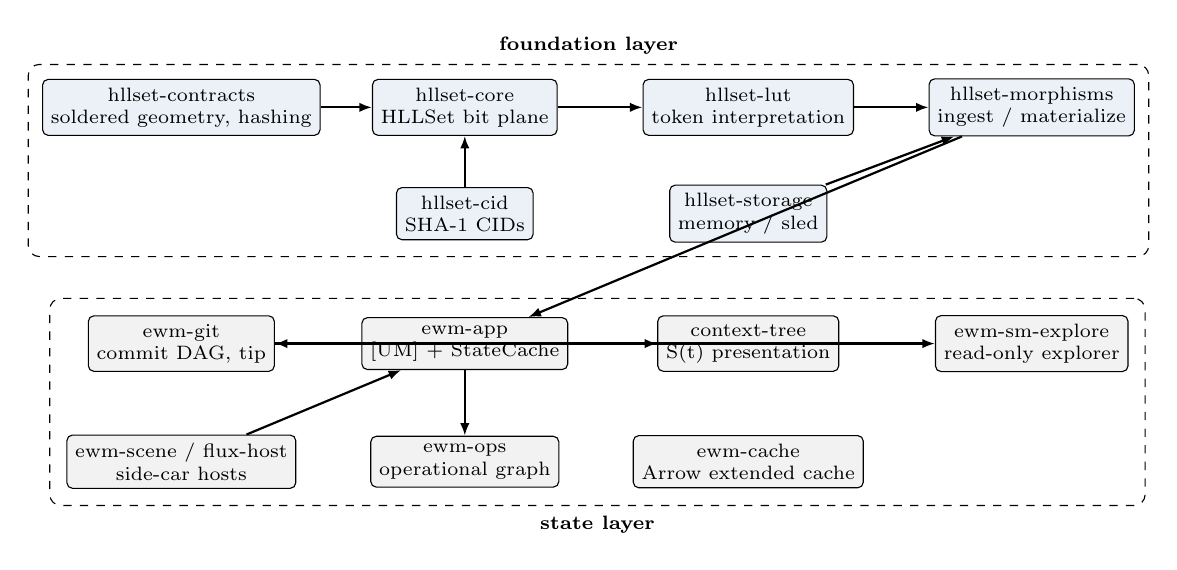
\begin{tikzpicture}[
  box/.style={draw, rounded corners=2pt, align=center, inner sep=3pt, font=\scriptsize},
  found/.style={box, fill=hlblue!8},
  state/.style={box, fill=black!5},
  arr/.style={-{Latex[length=1.6mm]}, thick}
]
\node[found] (contracts) at (0,0)      {hllset-contracts\\ soldered geometry, hashing};
\node[found] (core)      at (3.6,0)    {hllset-core\\ HLLSet bit plane};
\node[found] (lut)       at (7.2,0)    {hllset-lut\\ token interpretation};
\node[found] (morph)     at (10.8,0)   {hllset-morphisms\\ ingest / materialize};
\node[found] (cid)       at (3.6,-1.35){hllset-cid\\ SHA-1 CIDs};
\node[found] (storage)   at (7.2,-1.35){hllset-storage\\ memory / sled};

\node[state] (git)     at (0,-3.0)    {ewm-git\\ commit DAG, tip};
\node[state] (app)     at (3.6,-3.0)  {ewm-app\\ {[UM]} + StateCache};
\node[state] (tree)    at (7.2,-3.0)  {context-tree\\ S(t) presentation};
\node[state] (explore) at (10.8,-3.0) {ewm-sm-explore\\ read-only explorer};
\node[state] (scene)   at (0,-4.5)    {ewm-scene / flux-host\\ side-car hosts};
\node[state] (ops)     at (3.6,-4.5)  {ewm-ops\\ operational graph};
\node[state] (cache)   at (7.2,-4.5)  {ewm-cache\\ Arrow extended cache};

\draw[arr] (contracts) -- (core);
\draw[arr] (core) -- (lut);
\draw[arr] (lut) -- (morph);
\draw[arr] (cid) -- (core);
\draw[arr] (storage) -- (morph);
\draw[arr] (morph) -- (app);
\draw[arr] (app) -- (git);
\draw[arr] (app) -- (tree);
\draw[arr] (git) -- (explore);
\draw[arr] (app) -- (ops);
\draw[arr] (scene) -- (app);
\begin{scope}[on background layer]
  \node[draw, dashed, rounded corners, fit=(contracts)(core)(lut)(morph)(cid)(storage), inner sep=5pt,
        label={[font=\scriptsize\bfseries]above:foundation layer}] {};
  \node[draw, dashed, rounded corners, fit=(git)(app)(tree)(explore)(scene)(ops)(cache), inner sep=6pt,
        label={[font=\scriptsize\bfseries]below:state layer}] {};
\end{scope}
\end{tikzpicture}
\caption{The two layers. The foundation layer knows only HLLSets and morphisms
(no notion of a ``turn'' or a ``world''); the state layer builds the machine on
top.}
\label{fig:layers}
\end{figure}

\begin{table}[t]
\centering
\small
\begin{tabular}{@{}p{0.30\textwidth}p{0.62\textwidth}@{}}
\toprule
Crate & Responsibility \\
\midrule
\texttt{hllset-contracts} & soldered invariants: $\Prec=10$, $\Reg=1024$, $\Bits=32$, MurmurHash3, bit addresses \\
\texttt{hllset-core} & the HLLSet bit plane (a Roaring bitmap) and its set algebra \\
\texttt{hllset-lut} & the LUT lattice: token interpretation, content-addressed \\
\texttt{hllset-morphisms} & \texttt{ingest} / \texttt{materialize} and the default API \\
\texttt{hllset-cid}, \texttt{hllset-storage} & CIDs; memory and sled persistence \\
\texttt{ewm-git} & the committed stack: commit DAG, tip, recovery \\
\texttt{ewm-app} & the stateless [UM] harness and the shared \texttt{StateCache} \\
\texttt{context-tree} & Merkle tree over the working set, the $S(t)$ presentation \\
\texttt{ewm-scene} & LLM$\leftrightarrow$HLLSet side-car helper (direct morphisms) \\
\texttt{ewm-flux-host} & side-car host adapter for a rectified-flow sampler \\
\texttt{ewm-ops} & content-addressed operational graph (value / program lattice) \\
\texttt{ewm-cache} & Arrow-backed extended cache (IPC spill/restore) \\
\texttt{ewm-sm-explore} & read-only explorer of the three-layer state \\
\bottomrule
\end{tabular}
\caption{Implementation map. The foundation layer is vocabulary-agnostic; the
state layer is where the machine lives.}
\label{tab:crates}
\end{table}

\subsection{The side-car loop}

A host model (an LLM, an OCR encoder, a vision model, a planner) is left
untouched. The state layer attaches beside it:

\begin{center}
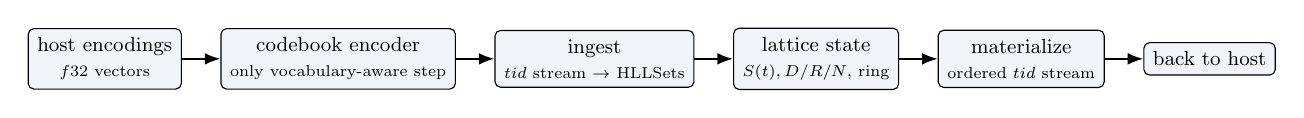
\begin{tikzpicture}[
  node distance=6mm, scale=0.82, transform shape,
  b/.style={draw, rounded corners=2pt, align=center, inner sep=4pt, font=\small, fill=hlblue!6},
  a/.style={-{Latex[length=2mm]}, thick}
]
\node[b] (enc) {host encodings\\ \scriptsize $f32$ vectors};
\node[b, right=of enc] (codec) {codebook encoder\\ \scriptsize only vocabulary-aware step};
\node[b, right=of codec] (ing) {ingest\\ \scriptsize $tid$ stream $\to$ HLLSets};
\node[b, right=of ing] (lat) {lattice state\\ \scriptsize $S(t), D/R/N$, ring};
\node[b, right=of lat] (mat) {materialize\\ \scriptsize ordered $tid$ stream};
\node[b, right=of mat] (back) {back to host};
\draw[a] (enc) -- (codec);
\draw[a] (codec) -- (ing);
\draw[a] (ing) -- (lat);
\draw[a] (lat) -- (mat);
\draw[a] (mat) -- (back);
\end{tikzpicture}
\end{center}

The encoder is the only vocabulary-aware step: it quantizes host encodings to a
shared codebook and emits \texttt{tid}$\{n\}$ tokens. Everything below it is
vocabulary-agnostic: any stream that can be tokenized can drive the same state
machine. This is what makes the layer a \emph{side-car} rather than a model: it
does not interpret content, it accumulates and reads structure.

\subsection{Store, cache, unit}

The state machine is one data structure over three locations:
\begin{itemize}[leftmargin=*,nosep]
  \item the \textbf{persistent store} (\texttt{ewm-git})---the committed stack,
    a content-addressed DAG whose head is the tip;
  \item the \textbf{shared cache} (\texttt{StateCache})---the emerging $S(t)$
    working set together with the materialized base $H(t{-}1)$;
  \item the \textbf{processing unit} (\texttt{ewm-app})---stateless and
    disposable, owning only a store handle, reading the tip, proposing the next
    state.
\end{itemize}
Caching and persistence are separated by content addressing: the cache is a pure
value, shareable between units, and rebuildable from the tip. A commit is the
atomic advance of the tip and records $H(t)$; a no-change pass commits nothing.
What the store actually persists is deliberately narrow---\emph{originals} and
\emph{base HLLSets}---with every compound held as a provenance-stamped view
and recomputed on read; \S\ref{sec:views} derives that discipline from the
change of basis.

% ============================================================================
\section{Transformations}
\label{sec:transforms}
% ============================================================================

\subsection{One turn}

A turn is the unit of transformation. Given a token list, the machine performs
the following steps; each step is a lattice operation, a Gaussian step, or a
commit.

\begin{enumerate}[leftmargin=*,nosep]
  \item \textbf{Encode.} Host encodings are quantized to a \texttt{tid} stream by
    the shared codebook encoder (the only vocabulary-aware step).
  \item \textbf{Ingest.} The stream is measured by the IICA morphism; the turn
    produces per-channel sketches. The current projection is the turn's
    \emph{original} $\HLL_\Tab$.
  \item \textbf{Join.} The working state advances by union:
    $S(t) \leftarrow S(t)\cup \HLL_\Tab$. Union is idempotent, commutative, and
    associative, so independent turns accumulate without coordination.
  \item \textbf{Ring push.} The original enters the ring (\S\ref{sec:ring});
    the push is one Gaussian step and returns novelty statistics.
  \item \textbf{Commit.} $H(t)$ is committed when the pass brings new bits
    \emph{or} the ring basis changed; a basis change alone is a structural
    commit.
  \item \textbf{Materialize.} On demand, bits are lowered back to tokens
    (LUT-first, probabilistic restoration) for the host.
\end{enumerate}

The $D/R/N$ decomposition is computed from $S(t)$ and $H(t{-}1)$ as in
Eq.~\eqref{eq:fundamental}. It is the per-transition reading that later frames
build on.

\subsection{The ring transformation}
\label{sec:ring}

The ring is the part of the machine that turns the sequence of originals into a
\emph{coordinate system}. We call the HLLSet a commit pushes its \emph{commit
HLLSet}, and an element of the ring basis a \emph{base HLLSet}. An HLLSet is a
subset of the bit plane and hence a
vector over $GF(2)$: symmetric difference is addition,
$x+x=0$, and intersection is multiplication, $x\cdot x=x$. The ring maintains a
\emph{basis} of the span of the originals---a row-echelon GF(2) basis with
distinct leading bits---and each original is reduced against it.

A push is one Gaussian step. Reducing the incoming original against the basis
either (i) returns zero, meaning the original is already an XOR of basis
elements (\emph{in span}), or (ii) leaves a non-zero \emph{residual}, which
becomes a new basis element with a new pivot. The basis change then has two
components, which the machine reports as \texttt{RingStats}:
\begin{itemize}[leftmargin=*,nosep]
  \item \textbf{extension}---the residual becomes a new direction (the span
    grows by one);
  \item \textbf{rotation}---every existing basis element containing the new
    pivot bit is re-pivoted by XOR with the residual, keeping leading bits
    distinct.
\end{itemize}
The number of re-pivoted elements is \texttt{rotation\_count}; the total Hamming
change of the old basis is
$\texttt{rotation\_mass} = \texttt{rotation\_count}\times\texttt{residual}$.
An in-span push changes nothing.

\subsection{A monotone basis and exact change of basis}
\label{sec:changeofbasis}

The ring keeps two roles separate: a \textbf{monotone basis} over
every commit HLLSet ever pushed, and a bounded \textbf{visibility window} of
recent commits used as context. Eviction moves the window; it never removes a
base HLLSet. Consequently the span is \emph{monotone},
\begin{equation}
\label{eq:monotone}
\spanof{B_1,\dots,B_k(t-1)} \;\subseteq\; \spanof{B_1,\dots,B_k(t)},
\end{equation}
and representability is non-decreasing: once a set is expressible as an XOR of
the basis, it remains so. Every commit HLLSet remains expressible in the base.

Because the span only grows, each old basis element has unique coordinates in
the new basis: the columns of a \textbf{change-of-basis matrix} $M$. A
coordinate vector $a$ at time $t{-}1$ transports to $a\cdot M$ at time $t$,
exactly. This is what keeps coordinates canonical across commits: the
coordinates of a fixed node change with the basis, but the change is a
deterministic, invertible (in the pure re-basis case) linear map, and the ring
stamps each basis with a \emph{generation} so stale projections can be
identified.

\begin{proposition}[Exact transport]
\label{prop:transport}
Let $B(t{-}1)$ and $B(t)$ be two bases of a monotone ring. Every basis element
of $B(t{-}1)$ has unique coordinates in $B(t)$, so any node expressible at
$t{-}1$ is expressible at $t$, and its coordinates transport by the
change-of-basis matrix.
\end{proposition}
\begin{proof}[Proof sketch]
Monotonicity gives $\spanof{B(t{-}1)}\subseteq\spanof{B(t)}$; coordinates are
unique because the basis is distinct for each commit; the transport is the
coordinate expansion of each affected old basis element in the new basis.
\end{proof}

\subsection{What the ring cannot do}

The ring span is a vector subspace over $GF(2)$: it is closed under symmetric
difference but \emph{not} under intersection, union, or difference. For
$A,B$ in the span,
\[
A\cup B = A\xor B\xor(A\cap B),
\qquad
A\setminus B = A\xor(A\cap B),
\]
so all three compounds lie in the same coset modulo the span and are
representable together or not at all. The meet is the single obstruction; a
general lattice expression is representable iff its meet content is. The exact
test for any node $X$ is $\res(X)=\emptyset$, equivalently
\texttt{coordinates}$(X)\neq\texttt{None}$. This is a feature, not a defect: it
gives a measurable quantity---how far a node is from being a linear combination
of the context.

\begin{remark}[Remainder, not canonical representative]
The reduction's remainder is deterministic for a fixed commit sequence but
is only \emph{a} representative of the coset $X+\spanof{B}$: the basis is
row-echelon without full reduction, and the reduction stops at the first
non-pivot leading bit. Congruent sets can return different remainders. The
coset-invariant fact---and the one the tests rely on---is
$\res(X)=\emptyset \Leftrightarrow X$ is in the span.
\end{remark}

\subsection{Views: originals, base HLLSets, and recreated compounds}
\label{sec:views}

The transport property is not only coordinate bookkeeping; it is the reason the
store keeps so little. Two kinds of node are \emph{materialized}:
\begin{itemize}[leftmargin=*,nosep]
  \item \textbf{originals}---the IICA sketches of measured token streams,
    content-addressed (\texttt{h:}$\langle$SHA-1$\rangle$) and immutable;
  \item \textbf{base HLLSets}---the monotone basis the ring produces,
    themselves content-addressed.
\end{itemize}
Everything else---unions $S(t)$, the $D/R/N$ components, residuals, soft keys,
covers, and projections---is a \textbf{view}: a node recorded as an
\emph{expression} over source nodes together with its \textbf{provenance}, the
ordered list of SHA-1 content identifiers of the HLLSets it is built from. A
view is not stored as a copy of its bits.

The reason is exactly that coordinates are basis-relative and the basis moves
(\S\ref{sec:rotating}): a compound frozen as a coordinate vector in one base, is different in another. The
correct rule is the transport of Proposition~\ref{prop:transport}---a reading is
valid only relative to the \emph{generation} of the basis it was taken in. So
the store keeps the recipe and its provenance, and the reader \emph{recreates}
the compound against the basis current at read time. Cache is the only place where compound HLLSets stay binary vectors.

Recreation is safe because the source nodes are IICA: the same recipe on the
same sources yields the same bits, so a view is deterministic and idempotent
under re-evaluation. It is also cheap: a view over $k$ base HLLSets costs a
handful of bit operations per base HLLSet, independent of how long the history
has grown. Caching is optional and subordinate---a materialized view may be
cached, but the cache entry is stamped with its basis generation, and a read in
a new generation re-projects only the entries queried, never the whole history
(the lazy back-propagated pattern used by the flow host). Storage is therefore
proportional to the number of \emph{originals} plus the size of the
\emph{base}, not to the number of compounds ever named---the operational form of
``discover, do not create.''

\begin{table}[t]
\centering
\small
\begin{tabular}{@{}p{0.28\textwidth}p{0.28\textwidth}p{0.36\textwidth}@{}}
\toprule
Node & Stored as & Read as \\
\midrule
original sketch & bits, \texttt{h:}$\langle$SHA-1$\rangle$ & itself \\
base HLLSet & bits, \texttt{h:}$\langle$SHA-1$\rangle$ & itself \\
union, $D/R/N$ & expression + provenance CIDs & recomputed against the read-time base \\
residual, soft key, cover, projection & expression + provenance + basis generation & recomputed; cached entries are generation-stamped \\
\bottomrule
\end{tabular}
\caption{What is stored and what is recomputed. Only originals and base
HLLSets are materialized; every compound is a provenance-stamped view that
is recreated against the base current at read time.}
\label{tab:views}
\end{table}

\begin{figure}[t]
\centering
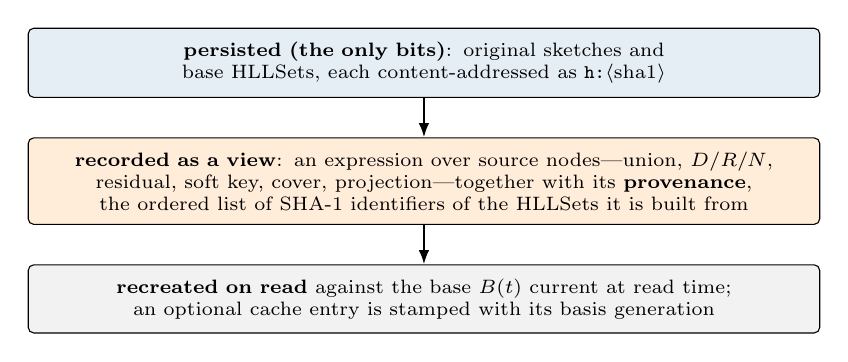
\begin{tikzpicture}[node distance=5mm,
  box/.style={draw, rounded corners=2pt, align=center, inner sep=5pt,
              font=\scriptsize, text width=0.80\textwidth},
  arr/.style={-{Latex[length=1.8mm]}, thick}]
\node[box, fill=hlblue!10] (mat)
  {\textbf{persisted (the only bits)}: original sketches and base HLLSets,
   each content-addressed as \texttt{h:}$\langle$sha1$\rangle$};
\node[box, fill=orange!15, below=of mat] (view)
  {\textbf{recorded as a view}: an expression over source nodes---union,
   $D/R/N$, residual, soft key, cover, projection---together with its
   \textbf{provenance}, the ordered list of SHA-1 identifiers of the HLLSets it
   is built from};
\node[box, fill=black!5, below=of view] (re)
  {\textbf{recreated on read} against the base $B(t)$ current at read time;
   an optional cache entry is stamped with its basis generation};
\draw[arr] (mat) -- (view);
\draw[arr] (view) -- (re);
\end{tikzpicture}
\caption{The storage discipline. Only originals and base HLLSets are
materialized; a compound is a view---a recipe plus provenance---and it is
recreated against the read-time base. Because the basis rotates, a stored
coordinate or bit copy would be stale; the recipe never is.}
\label{fig:views}
\end{figure}

A view record therefore carries no bits of its own; an abbreviated example:

\begin{quote}\small
\begin{verbatim}
{
  "view":              "p:9f2c1d...",        # id of the recipe, not the result
  "expr":              "union",              # or drn | residual | project | ...
  "sources":           ["h:1a7e...", "h:4b02...", "h:cd91..."],
  "basis_generation":  37,                   # generation the reading was taken in
  "materialized":      false                 # recomputed on read
}
\end{verbatim}
\end{quote}

% ============================================================================
\section{Trajectory}
\label{sec:trajectory}
% ============================================================================

The trajectory is the sequence of readings of the state. A \emph{frame} is a
named set of dimensions $D=(D_1,\dots,D_m)$; the frame's coordinate map is
\begin{equation}
\label{eq:frame}
\varphi_D(X) = \bigl(\,\BSS(X,D_1),\dots,\BSS(X,D_m)\,\bigr),
\qquad
\BSS(X,D_i) = \frac{|X\cap D_i|}{|D_i|},
\end{equation}
and $\varphi_D(X(t))$ over $t$ is the HLLSet trajectory in that frame. Different
frames are different readings of the same nodes: $D/R/N$ is the temporal frame,
the ring basis is the linear frame, joined perceptrons are the structural frame,
and a codebook gate is a per-user frame. Varying the frame changes what we see,
not what the state is.

\subsection{Signals}

Four families of trajectory signals are used in the experiments and the host
loops.
\begin{itemize}[leftmargin=*,nosep]
  \item \textbf{Linear novelty (residual).} $\res(X)$ is the part of $X$ outside
    the ring span: what no XOR of originals can express. Its popcount is a
    higher-order $N$---it asks ``what cannot be assembled from the context,''
    where the bit-level $N=S(t)\setminus H(t{-}1)$ asks ``which bits are new.''
  \item \textbf{Rotation.} \texttt{rotation\_count} counts how many existing
    directions re-index themselves through a new one; it is zero whenever the
    residual is zero, and among novel frames it measures the re-indexing cost.
  \item \textbf{Bit novelty (cover).} The \emph{cover} of the basis is the union
    of its elements; the identity $\bigcup_i B_i = \bigcup_j (\text{originals})_j$
    holds exactly, because an XOR is a subset of a union and every base HLLSet
    is an XOR of the commit HLLSets. The bit novelty $N_{\mathrm{bit}}=X\setminus\mathrm{cover}$
    is the part no span member can contain; it satisfies
    $N_{\mathrm{bit}}\subseteq \res(X)$.
  \item \textbf{Basis frames (time travel).} Every frame is also projected into
    the first recorded basis, with a \emph{spill}
    $|X\setminus \mathrm{cover}(F_0)|$ measuring the error of reading the present
    through the past's lens.
\end{itemize}

\subsection{A toolkit with labeled exactness}

The companion note and the notebooks develop a small toolkit over the ring and
the lattice. Its exactness is part of its specification (Table~\ref{tab:tools}).

\begin{table}[t]
\centering
\small
\begin{tabular}{@{}p{0.24\textwidth}p{0.68\textwidth}@{}}
\toprule
Tool & Exactness \\
\midrule
change of basis $B(t{-}1)\to B(t)$ & exact GF(2) matrix; coordinates transport by $a\cdot M$ \\
BSS transform $\BSS(t{-}1)\to\BSS(t)$ & \emph{not} linear (XOR vs.\ $\cap$); exact by re-projection, or by the meet-order ladder ($\text{order}\ge$ support size); new directions must be measured, not rotated \\
cover identity & exact: $\bigcup$basis $=\bigcup$originals \\
projection $X\mapsto(D,R,N)$ onto the cover & exact lattice operations; $N\subseteq\res(X)$ \\
minimal cover & unique coordinate support when in span; greedy $H(d)$-approximate union cover otherwise \\
\bottomrule
\end{tabular}
\caption{Trajectory tools and their exactness. The one place to be careful is the
BSS transform: a BSS vector is not a sufficient state to rotate exactly; the
exact alternative is re-projection, and the nonlinearity is the meet
obstruction of \S\ref{sec:changeofbasis}.}
\label{tab:tools}
\end{table}

\subsection{Reading the trajectory}

Figure~\ref{fig:trajectory} sketches the trajectory picture: nodes advance by
join and commit; the ring basis grows; each turn contributes a novelty reading.
The machine exposes the trajectory in three locational views (run-time $S(t)$,
cache, committed store) and in any named frame.

\begin{figure}[t]
\centering
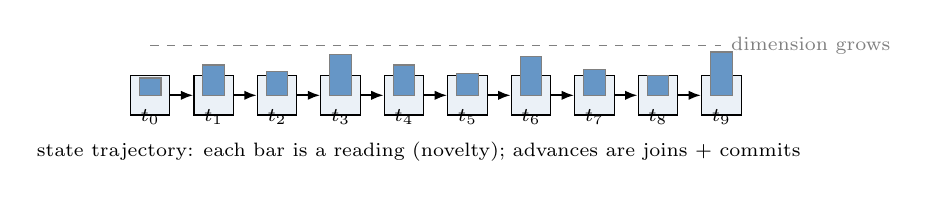
\begin{tikzpicture}[x=0.62cm,y=0.55cm,
  st/.style={draw, fill=hlblue!8, minimum width=5mm, minimum height=5mm, font=\scriptsize},
  a/.style={-{Latex[length=1.6mm]}, thick}]
\foreach \i/\h in {0/0.4,1/0.7,2/0.55,3/0.95,4/0.7,5/0.5,6/0.9,7/0.6,8/0.45,9/1.0}{
  \node[st] (s\i) at (\i*1.3,0) {};
  \fill[hlblue!60] (\i*1.3-0.22,0) rectangle (\i*1.3+0.22,\h);
  \draw[gray] (\i*1.3-0.22,0) rectangle (\i*1.3+0.22,\h);
  \node[font=\scriptsize] at (\i*1.3,-0.5) {$t_{\i}$};
  \ifnum\i>0 \draw[a] (s\the\numexpr\i-1) -- (s\i); \fi
}
\draw[dashed, gray] (0,1.15) -- (11.7,1.15) node[right,font=\scriptsize]{dimension grows};
\node[align=center,font=\scriptsize] at (5.5,-1.3)
  {state trajectory: each bar is a reading (novelty); advances are joins + commits};
\end{tikzpicture}
\caption{The state trajectory. Nodes advance by join; the ring basis grows
monotonically; each turn contributes a novelty reading. Spikes mark transitions
(the synthetic clip's scene cuts in \S\ref{sec:experiments}).}
\label{fig:trajectory}
\end{figure}

% ============================================================================
\section{Rotating coordinates and the top-state decomposition}
\label{sec:rotating}
% ============================================================================

The ring's basis is not a fixed frame. Each commit appends a commit HLLSet
(extension) and re-pivots some existing ones (rotation), so the basis
$B(t)=\{B_1(t),\dots,B_{k(t)}(t)\}$ \emph{moves}. A node that does not change
still changes its coordinates; the transport of
Proposition~\ref{prop:transport} is exactly the bookkeeping for that motion.
Over the $10\times10$ clip the basis re-pivots $534$ coordinates in $100$
commits (a mean of $5.34$ per commit), so the frame is moving on almost every
step.

\subsection{Decomposing the top state}

Let $U(t)$ be the \emph{top state} of commit $t$: the union of the commit's
perceptron sketches (in the single-stream clip, simply the frame sketch
$X(t)$). We read it in the coordinates that were current when it arrived,
$B(t{-}1)$---the context it is measured against---and obtain three exact
objects:
\begin{itemize}[leftmargin=*,nosep]
  \item the \textbf{soft key}, the lattice projection onto each base
    coordinate,
    \[
    w_i(t)=\frac{|U(t)\cap B_i(t{-}1)|}{|B_i(t{-}1)|}\in[0,1],
    \]
    always defined, whether or not $U(t)$ is in the span;
  \item the \textbf{hard key}, the unique coordinate vector $c(t)$ with
    $U(t)=\xor_i c_i\,B_i(t{-}1)$, defined exactly when
    $\res_{B(t{-}1)}(U(t))=\emptyset$;
  \item the \textbf{residual} $\res_{B(t{-}1)}(U(t))$, the off-span part, which
    completes the exact decomposition
    \[
    U(t)=P(t)\;\xor\;\res_{B(t{-}1)}(U(t)),
    \qquad
    P(t)=\xor_{i:\,c_i=1} B_i(t{-}1).
    \]
\end{itemize}

The soft key says \emph{where} the new state lands in the current coordinates;
the hard key says whether it lies entirely inside them; the residual says how
much of it cannot be expressed by them at all. On the clip no top state is
fully inside the prior span ($0/100$): every frame carries new drift, so the
hard key is usually absent and the residual is the informative object. The mean
soft-key entry is $0.091$ with a maximum of $0.804$---most coordinates are
barely touched, a few carry the frame---and the pre-commit residual averages
$612.6$ bits at the nine scene cuts against $328.3$ bits in scenes
($1.9\times$).

\subsection{The coordinate--time matrix}

Arranging the soft keys into a matrix $W\in\mathbb{R}^{T\times k}$, with base
coordinates on the $Y$ axis and commits on the $X$ axis, makes the trajectory
readable in one picture (Figure~\ref{fig:rotating}). Three structures are
visible at once:
\begin{itemize}[leftmargin=*,nosep]
  \item the \textbf{frontier}---the white line of the span dimension---grows
    monotonically and bounds the region where no coordinate exists yet;
  \item \textbf{rows} are born as coordinates appear and then evolve: a bright
    row is a direction that stays aligned with many commits (a stable context
    direction); a row that dims has been rotated away from current content;
  \item the \textbf{residual} panel spikes at transitions, giving a
    representation-independent event signal.
\end{itemize}

\begin{figure}[t]
\centering
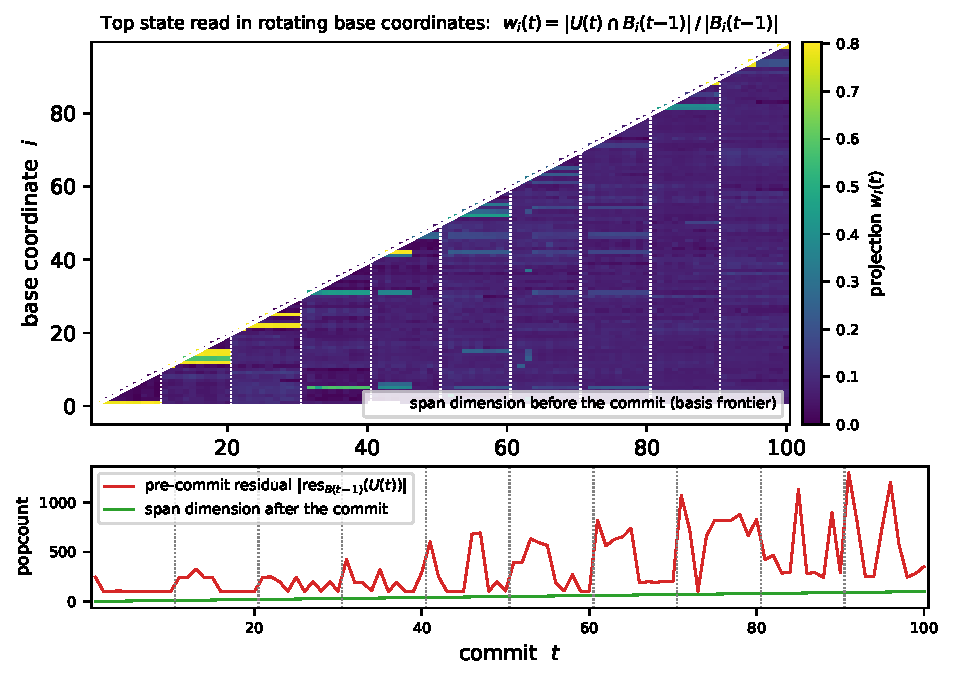
\includegraphics[width=\textwidth]{figures/rotating_coordinates.pdf}
\caption{The trajectory in rotating base coordinates on the $10\times10$ clip.
Top: the soft key $w_i(t)$ of each commit's top state in the coordinates
$B(t{-}1)$ current when it arrived (rows are base coordinates in creation
order; the white line is the span frontier; dotted lines are scene cuts).
Bottom: the pre-commit residual and the span dimension. Rows are born as the
basis grows, the frame re-pivots throughout, and the residual spikes at every
scene cut.}
\label{fig:rotating}
\end{figure}

\begin{remark}[The cumulative union projects to $1$]
It is tempting to project the \emph{cumulative} union of all HLLSets onto the
base coordinates. That projection is uninformative: every base HLLSet is an XOR
of commit HLLSets, hence a subset of the cumulative union, so
$|\bigcup_{\tau\le t}U(\tau)\cap B_i(t)|/|B_i(t)|=1$ for every coordinate---we
measure exactly $1.000$ for all of them on the clip. The informative object is
the \emph{per-commit} top state (or its novel part), which is what
Figure~\ref{fig:rotating} shows.
\end{remark}

\subsection{Reading it in practice}

The rotating-coordinate view turns the toolkit of Table~\ref{tab:tools} into
trajectory readings. Coordinates with consistently high soft keys are the
stable directions a context can be compressed to (the minimal cover);
coordinates that spike and then fade mark transitions; and the residual is the
novelty that no combination of current coordinates can express. Because the
frame moves, a reading is comparable to another reading only once it is stamped
with its basis generation---which is exactly what the ring records.

% ============================================================================
\section{Experimental illustration}
\label{sec:experiments}
% ============================================================================

We exercise the machine on a synthetic clip with known structure: $10$ scenes
$\times$ $10$ frames, where each frame holds a $200$-token scene vocabulary plus
$56$ tokens of per-frame drift. Scene cuts start at frames $11,21,\dots,91$; a
window of frames shares vocabulary, and a cut introduces a new one. The clip is
analyzed incrementally as frames arrive. The measurements below are reproduced
by the notebooks in the repository (a bit-exact Python mirror of the ring on
real HLLSets), and by the Rust implementation's own test suite.

\subsection{Novelty detects the transitions}

\begin{table}[t]
\centering
\small
\begin{tabular}{@{}lrrr@{}}
\toprule
Signal (morphism, mode) & cut mean & in-scene mean & separation \\
\midrule
linear residual, windowed ($\mu_{ng}$)~\cite{companion2026} & $782.9$ & $271.4$ & $2.9\times$ \\
linear residual, monotone ($\mu_{\mathrm{flat}}$) & $612.6$ & $328.3$ & $1.9\times$ \\
bit novelty $N$, monotone ($\mu_{\mathrm{flat}}$) & $99.0$ & $26.4$ & $3.75\times$ \\
\bottomrule
\end{tabular}
\caption{Novelty at scene cuts vs.\ in-scene drift. The windowed linear residual
is the sharpest linear signal on the production $n$-gram morphism (all $9/9$
cuts above in-scene mean $+2\sigma$); the bit-novelty $N=X\setminus\mathrm{cover}$
is the sharpest signal on the flat-morphism clip. The two morphisms are
different measurements and their scales are not comparable; the structural
conclusions are morphism-agnostic.}
\label{tab:cuts}
\end{table}

The linear residual is a higher-order $N$: it spikes when a frame cannot be
assembled from anything the context has seen. The bit novelty $N$ is the exact
lattice part no span member can contain. Both flag the transitions; $N$ is the
more robust reading on the synthetic clip because it is bounded by the cover and
does not accumulate re-indexable bits.

\subsection{Representability is measurable}

The ring's representability laws are not asymptotic statements; they are
measured exactly on the clip (Table~\ref{tab:repr}). Over $394$ frame pairs,
symmetric differences are \emph{always} in the span, while intersections,
unions, and differences are \emph{never} in it for this data; the three
compounds are pairwise congruent modulo the span in every case. The meet is the
obstruction, exactly as \S\ref{sec:changeofbasis} predicts. The change of basis
between two commits is sparse (density $0.038$), all $50$ old basis elements are
representable in the later $100$-dimensional basis, and the coordinate
round-trip is the identity---the practical content of
Proposition~\ref{prop:transport}.

\begin{table}[t]
\centering
\small
\begin{tabular}{@{}lr@{}}
\toprule
Measured on the $10\times10$ clip & Result \\
\midrule
$A\xor B$ in span & $394/394$ \\
$A\cap B$, $A\cup B$, $A\setminus B$ in span & $0/394$ \\
$\cap,\cup,\setminus$ pairwise congruent mod span & $394/394$ \\
change-of-basis density (50 $\to$ 100) & $0.038$ \\
old basis elements representable after extension & $50/50$ \\
coordinate transport round-trip & identity \\
cover identity $\bigcup$basis $=\bigcup$originals & holds (monotone and windowed) \\
\bottomrule
\end{tabular}
\caption{Representability and transport, measured. The ring is a lossy linear
projection of the lattice; the residual is the exact error of that projection.}
\label{tab:repr}
\end{table}

\subsection{Trajectory tools}

The toolkit of Table~\ref{tab:tools} is exercised end-to-end. The change of
basis transports coordinates exactly; the BSS transform is shown to be
nonlinear (a two-element overlap example predicts $1.00$ where the exact
re-projection is $0.00$), and exact by the meet-order ladder when the order
reaches the support size; the cover identity holds in both monotone and windowed
modes; the projection $(D,R,N)$ reassembles the frame and satisfies
$N\subseteq\res(X)$; and the minimal cover compresses a five-frame context of
$442$ bits into $12$ basis elements with full coverage, with the residual as the
irreducible remainder.

\begin{remark}[What the numbers say about the architecture]
The machine's central quantity---the residual---is not a heuristic score bolted
onto a buffer; it is the distance from a node to the span of the context, and it
is computable exactly, incrementally, and cheaply (a handful of bit operations
per basis element). The trajectory is therefore auditable: every reading can be
recomputed from the committed originals.
\end{remark}

% ============================================================================
\section{Related work}
\label{sec:related}
% ============================================================================

\paragraph{Sketches and cardinality.} HLLSets descend from probabilistic
cardinality estimation~\cite{flajolet2007,bloom1970} and resemblance
sketches~\cite{broder1997}. Our use is different: we do not estimate
cardinality; we use the sketch as a \emph{state} and its lattice as the algebra
of transitions. The soldered geometry fixes a common plane so that set
operations are exact bit operations.

\paragraph{Content-addressed storage and histories.} Content addressing is the
basis of Merkle trees~\cite{merkle1988}, Git~\cite{git}, and
IPFS/IPLD~\cite{benet2014}. The state machine reuses the idea at the level of
\emph{state}: the tip of a commit DAG is the state, and recovery is a read, not
a replay. Merging independent contributions is a join, which relates the
approach to CRDTs~\cite{shapiro2011}; here the join is set union on a shared
bit plane, and idempotence comes from IICA rather than from a merge function.

\paragraph{World models and memory for models.} World models learn a predictive
latent state~\cite{ha2018}; JEPA-style architectures separate encoder, context,
and predictor~\cite{lecun2022}; retrieval-augmented systems attach a memory to
a model~\cite{lewis2020}. Our side-car is orthogonal: it does not learn the
world, it \emph{holds} the state as a lattice node and advances it by
transformation. The predictor layer is pluggable and lives above the state
layer, not inside it.

% ============================================================================
\section{Discussion and limitations}
\label{sec:discussion}
% ============================================================================

\paragraph{No canonical basis.} GF(2) has no canonical basis; the ring's basis
depends on ingestion order and pivot choice. Coordinates therefore mean
something inside one commit sequence. A canonical alternative---the atoms of
the Boolean algebra generated by the originals---is exponential in the number
of commit HLLSets and is not used. The monotone basis makes coordinates comparable
across a run but not across different ingestion orders.

\paragraph{The remainder is not canonical.} The residual is a coset
representative, not a canonical one; congruent sets may leave different
remainders. The invariant is the coset, and the zero test is the exact
representability criterion. Trajectory signals built from the residual should be
read as representatives, not as unique values.

\paragraph{Monotone growth has a cost.} Keeping every commit HLLSet makes
representability monotone and removes eviction churn, but the span dimension
grows with the history, and coordinates grow with it. The windowed mode bounds
the visibility (and hence the per-frame readings) at the cost of losing
representability of evicted originals. The two modes are a deliberate trade;
the experiments report both.

\paragraph{Union identities survive only as inclusions.} The production
$n$-gram morphism is inclusion-isotonic but not a join homomorphism, so some
union identities hold as inclusions rather than equalities. The structural
results---$\xor$ closure, the meet obstruction, the cover identity---hold in the
image of whichever IICA morphism is chosen.

\paragraph{Recomputation is the price of correctness.} Keeping only originals
and base HLLSets makes stale-coordinate bugs structurally impossible, but
every read of a compound pays its expression cost (a handful of bit operations
per base HLLSet). The mitigation is generation-stamped caching---not storing
compounds---and the open question is the cache policy that keeps the read cost
flat as the base grows.

% ============================================================================
\section{Conclusion and future work}
\label{sec:conclusion}
% ============================================================================

We presented a state machine whose state is a content-addressed HLLSet and whose
transformations are lattice operations. The design separates the emerging state
$S(t)$, the committed base $H(t{-}1)$, and the per-transition decomposition
$D/R/N$; a stateless processing unit proposes transitions, a shareable cache
holds the working state, and a content-addressed store makes the trajectory
durable and replayable. The ring transformation gives the trajectory a
coordinate system that is deterministic per commit sequence and monotone
across commits, together with novelty signals that detect transitions exactly
and cheaply.

Several directions follow directly. First, a \textbf{trajectory-stability
study}: the coordinate--time matrix of \S\ref{sec:rotating} can be analyzed as
a time series (row birth, drift, and death) to identify stable context
directions automatically and to predict transitions from early-warning signals
in the soft keys. Second, a
\textbf{multi-world} extension: the hash configuration is a parameter of the
measurement, so independent users can share one lattice while reading it through
different interpretations; the companion note develops the isolation and bridge
theory. Third, a \textbf{closed loop}: the trajectory readings already drive a
controller in our host experiments (memory plus curiosity), and the residual and
bit-novelty signals are natural reward and surprise channels. Fourth, a
\textbf{scaled evaluation} on real, long-horizon model streams with the same
protocol used here. The engineering claim we make is deliberately modest and
testable: any token-producing model can be given a state that is cheap to
advance, exact to compare, and safe to replay.

% ============================================================================
\section*{Acknowledgment}
% ============================================================================
This article was written in collaboration between the authors and an AI
assistant, following the practice of the companion note. The human authors
developed the EWM framework, the HLLSet algebra, and the
\texttt{ewm-state-machine} realization, and directed the line of argument; the
AI assistant helped to draft and structure the text, work through the formal
statements, and verify the correspondence with the implementation. The
conceptual content is the authors' own.

% ============================================================================
\appendix
\section{Implementation map}
% ============================================================================

\begin{table}[h]
\centering
\small
\begin{tabular}{@{}p{0.34\textwidth}p{0.58\textwidth}@{}}
\toprule
Concept & Artifact \\
\midrule
bit plane, HLLSet & \texttt{hllset-core::HLLSet} (Roaring bitmap) \\
geometry $\Prec,\Reg,\Bits$ & \texttt{hllset-contracts} (\texttt{P}, \texttt{M}, \texttt{BITS\_PER\_REG}) \\
bit address & \texttt{hllset-contracts::BitAddress} \\
morphism $\mu$ & \texttt{hllset-morphisms::ingest / materialize} \\
turn & \texttt{ewm-app::run\_turn} \\
working state $S(t)$ & \texttt{ewm-app::StateCache::working} \\
base $H(t{-}1)$ & commit tip (\texttt{ewm-git}) \\
$D/R/N$ & \texttt{ewm-scene::noether} and the commit decomposition \\
ring basis, push & \texttt{ewm-boolring::BoolWindow} \\
ring stats & \texttt{RingStats\{residual, in\_span, dimension, rotation\_count, rotation\_mass\}} \\
commit DAG, tip & \texttt{ewm-git} (\texttt{commit}, \texttt{head}) \\
$S(t)$ presentation & \texttt{context-tree} (Merkle tree over turn leaves) \\
side-car hosts & \texttt{ewm-scene} (LLM), \texttt{ewm-flux-host} (flow) \\
operational graph & \texttt{ewm-ops} (value / program lattice) \\
originals, base HLLSets & content-addressed HLLSet nodes (\texttt{h:}$\langle$sha1$\rangle$) \\
view (recipe + provenance) & \texttt{ewm-ops} program lattice (\texttt{p:}$\langle$sha1$\rangle$), vocabulary (\texttt{v:}$\langle$sha1$\rangle$); provenance is the list of source \texttt{h:} CIDs \\
explorer & \texttt{ewm-sm-explore} \\
\bottomrule
\end{tabular}
\caption{Concept-to-code correspondence.}
\label{tab:impl}
\end{table}

\begin{thebibliography}{99}
\bibitem{companion2026} A.~Mylnikov, A.~Mylnikov Jr., and D.~Kumar,
\textit{The EWM Lattice and Its Worlds: HLLSets, Emerging Lattices, and
Multi-World Representation}, companion note to \textit{Emerging World Models},
2026.

\bibitem{ewm2026} A.~Mylnikov and D.~Kumar, \textit{Emerging World Models: A
Structural Framework for Self-Organizing World Representations}, consolidation
document, August 2026.

\bibitem{astesj2026} \textit{HLLSet Algebra: A Content-Addressed Set Algebra for
Emergent Ontology}, ASTES Journal, 2026.

\bibitem{birkhoff1940} G.~Birkhoff, \textit{Lattice Theory}, American
Mathematical Society Colloquium Publications, 1940.

\bibitem{flajolet2007} P.~Flajolet, \'E.~Fusy, O.~Gandouet, and F.~Meunier,
\textit{HyperLogLog: the analysis of a near-optimal cardinality estimation
algorithm}, in \textit{Analysis of Algorithms (AofA)}, 2007.

\bibitem{bloom1970} B.~H.~Bloom, \textit{Space/time trade-offs in hash coding
with allowable errors}, Communications of the ACM, 1970.

\bibitem{broder1997} A.~Z.~Broder, \textit{On the resemblance and containment of
documents}, in \textit{Compression and Complexity of Sequences}, 1997.

\bibitem{murmur3} A.~Appleby, \textit{MurmurHash3}, 2011; x64-128 variant, lower
64 bits, configurable seed.

\bibitem{merkle1988} R.~C.~Merkle, \textit{A digital signature based on a
conventional encryption function}, in \textit{Advances in Cryptology
(CRYPTO)}, 1988.

\bibitem{git} S.~Chacon and B.~Straub, \textit{Pro Git}, Apress, 2nd ed., 2014.

\bibitem{benet2014} J.~Benet, \textit{IPFS---Content Addressed, Versioned,
P2P File System}, arXiv:1407.3561, 2014.

\bibitem{shapiro2011} M.~Shapiro, N.~Pregui\c{c}a, C.~Baquero, and
M.~Zawirski, \textit{Conflict-free replicated data types}, in \textit{Symposium
on Self-Stabilizing Systems (SSS)}, 2011.

\bibitem{ha2018} D.~Ha and J.~Schmidhuber, \textit{World Models}, arXiv:1803.10122,
2018.

\bibitem{lecun2022} Y.~LeCun, \textit{A Path Towards Autonomous Machine
Intelligence}, OpenReview, 2022.

\bibitem{vaswani2017} A.~Vaswani et al., \textit{Attention is all you need}, in
\textit{Advances in Neural Information Processing Systems (NeurIPS)}, 2017.

\bibitem{lewis2020} P.~Lewis et al., \textit{Retrieval-augmented generation for
knowledge-intensive NLP tasks}, in \textit{NeurIPS}, 2020.

\bibitem{ashby1952} W.~R.~Ashby, \textit{Design for a Brain}, Chapman \& Hall,
1952.

\bibitem{lemire2018} D.~Lemire, O.~Kaser, N.~Kurz, L.~Deri, C.~O'Hara,
F.~Saint-Jacques, and G.~Ssi-Yan-Kai, \textit{Roaring bitmaps: implementation of
an optimized software library}, Software: Practice and Experience, 2018.
\end{thebibliography}

\end{document}
